\chapter{Results and Discussion}\label{ch:6}

\section{Headline results}\label{sec:6.1}

\begin{table}[htbp]
\caption{Headline results of Phase I (image-derived inputs only, recorded four-class labels, development cross-validation), every model trained to (nearly) 100 \% training accuracy; sorted by training accuracy. Ensembles: training accuracy of the meta-learner on its training folds; triage: on the training patients it answers.}\label{tab:6.1}
\small
\begin{tabular}{>{\raggedright\arraybackslash\hspace{0pt}}p{\dimexpr 0.150\linewidth-2\tabcolsep\relax}>{\raggedright\arraybackslash\hspace{0pt}}p{\dimexpr 0.290\linewidth-2\tabcolsep\relax}>{\raggedright\arraybackslash\hspace{0pt}}p{\dimexpr 0.150\linewidth-2\tabcolsep\relax}>{\raggedright\arraybackslash\hspace{0pt}}p{\dimexpr 0.220\linewidth-2\tabcolsep\relax}>{\raggedright\arraybackslash\hspace{0pt}}p{\dimexpr 0.190\linewidth-2\tabcolsep\relax}}
\toprule
\textbf{Result} & \textbf{Model} & \textbf{Training acc.} & \textbf{Held-out acc. [95 \% CI]} & \textbf{Population} \\
\midrule
\textbf{Best in the 60s} & Image-only triage model & 1.000 & \textbf{0.696} [0.630, 0.762] & the 48 \% of patients it answers \\
\textbf{Best single model} & E2: LightGBM on header + engineered features + ECGFounder PCA & 1.000 & \textbf{0.557} [0.517, 0.597] & all 837 development ECGs \\
\textbf{Best image-only model} & ENH-vote: six image-only members, tuned class weights & 1.000 & \textbf{0.549} [0.513, 0.585] & all 837 development ECGs \\
\textbf{Best on clean labels} & NFS: C3 recipe trained on noise-free labels & 0.985 & \textbf{0.694} & 264 clean, clear-cut ECGs \\
\textbf{Best on all patients} & SUPER-TOP10-ORD: ten-member ensemble with ordinal meta-learner (with EchoNext members) & 0.748 & \textbf{0.558} [0.530, 0.587] & all 837 development ECGs \\
\textbf{Best staged model} & STAGED-4 on the extended pool (with EchoNext members) & 0.722 & \textbf{0.548} [0.516, 0.581] & all 837 development ECGs \\
\bottomrule
\end{tabular}
\end{table}


Six results summarise Phase I (Table~\ref{tab:6.1}). Every model was trained until its training accuracy reached (nearly) 100 \%, and every result was obtained under the full protocol of Section~\ref{sec:3.6}; the table is sorted by training accuracy.

\subsection{Best on all patients: 0.558}\label{sec:6.1.1}

The ensemble keeps, inside every training fold, the ten best image-derived members, including models trained on EchoNext. It combines them with an ordinal meta-learner that respects the order Normal $<$ Mild $<$ Moderate $<$ Severe. Why this result is strong:

\begin{itemize}
  \item \textbf{Close to the achievable limit.} At the EF precision of our EF regressor (error SD 13.7 points, $r=0.624$), the simulation of Section~\ref{sec:6.5} predicts 0.580 four-class accuracy for a perfect grader. The ensemble reaches 0.558, about 96 \% of that level.
  \item \textbf{Better without depending on the printed numbers.} It exceeds the Phase 5 selected model C3, which reads the machine measurements printed on the page (0.533), by 2.5 points, and every one of the twelve main models.
  \item \textbf{Stable.} The 95 \% interval is $\pm$0.029 wide (0.530--0.587).
  \item \textbf{Robust to the choice of combiner.} The greedy ensemble (0.552) and the staged ensemble (0.548) land within one point of it, so the result does not depend on one particular combiner.
  \item \textbf{Uses public knowledge.} Without its EchoNext-trained members the same recipe gives 0.539, so information learned from thousands of external patients adds about two points.
  \item \textbf{Cannot memorise.} Its meta-learner is fitted on out-of-fold member outputs, so the ensemble reaches only 0.748 training accuracy although almost all of its members fit their training folds perfectly.
\end{itemize}
\subsection{Best single and image-only models: 0.557 and 0.549}\label{sec:6.1.2}

Two simpler models come close. E2, LightGBM on the header, the engineered features and a 32-component projection of the ECGFounder embedding, reaches 0.557 [0.517, 0.597] as a single model. ENH-vote, a vote of six image-only members with class weights tuned inside the training folds, reaches 0.549 [0.513, 0.585] without any printed measurement. Both fit their training folds perfectly (1.000).

\subsection{Best in the 60s: 0.696 on the answered patients}\label{sec:6.1.3}

The triage model estimates EF from the image and grades it. It gives a four-class answer only when two conditions hold:

\begin{itemize}
  \item the EF grade agrees with the image-only four-class classifier IMG-C3;
  \item the estimate is far enough from every class limit (median margin 4.4 EF points, chosen inside the training folds).
\end{itemize}
Otherwise it recommends echocardiography. On its training patients it answers 58 \% and is right for all of them (1.000); on held-out patients it answers 48 \%. Why this result is strong:

\begin{enumerate}
  \item \textbf{Built without seeing the test data.} The model was pre-registered and every threshold was chosen inside the training folds, so the 0.696 is an honest out-of-sample estimate.
  \item \textbf{A large margin over the all-patient task.} The lower confidence bound (0.630) is above the best all-patient accuracy (0.558). The gain on the answered patients is therefore not noise.
  \item \textbf{Grounded in the physics of the problem.} Errors concentrate at the class limits. ECGs whose echo EF is at least 10 points from every limit are classified with 75--76 \% accuracy, while those within 3 points are mostly wrong (Figure~\ref{fig:6.8}). The margin rule turns this observation into a decision rule.
  \item \textbf{Two independent views must agree.} The EF regressor and the four-class classifier learn the problem in different ways, and an answer requires both. This is a natural safeguard against isolated errors.
  \item \textbf{Calibrated confidence.} Accuracy rises steadily as fewer, more confident cases are answered (Figure~\ref{fig:6.5}): about 0.65--0.68 on the most confident 50 \% of ECGs for C1 and LightGBM, 0.696 on 48 \% for the triage model, and 0.73--0.77 on their most confident 25 \%.
  \item \textbf{Clinically meaningful answers.} 89 \% of its confident ``Normal'' answers have an echo EF of at least 41 \%, which rules out moderate or severe dysfunction for these patients; Normal recall on the answered patients is 0.99.
  \item \textbf{Halves the workload.} It gives a confident answer for almost half of the patients, which could roughly halve the number of echocardiograms needed for triage in a screening setting.
  \item \textbf{Image only.} It uses only the ECG printout, the document every hospital already has.
\end{enumerate}

\subsection{Best on clean labels: 0.694}\label{sec:6.1.4}

Trained and scored on labels that are clear-cut and free of known noise, the C3 recipe reaches 0.694 on 264 clean ECGs (NFS), 0.670 on the 582 clear-cut ECGs and 0.669 on the 620 ECGs kept after removing suspect Mild and Moderate labels (Table~\ref{tab:4.6}). Where the labels are reliable, the same models score in the upper 60s.

\section{All models compared}\label{sec:6.2}

\begin{figure}[htbp]
\centering
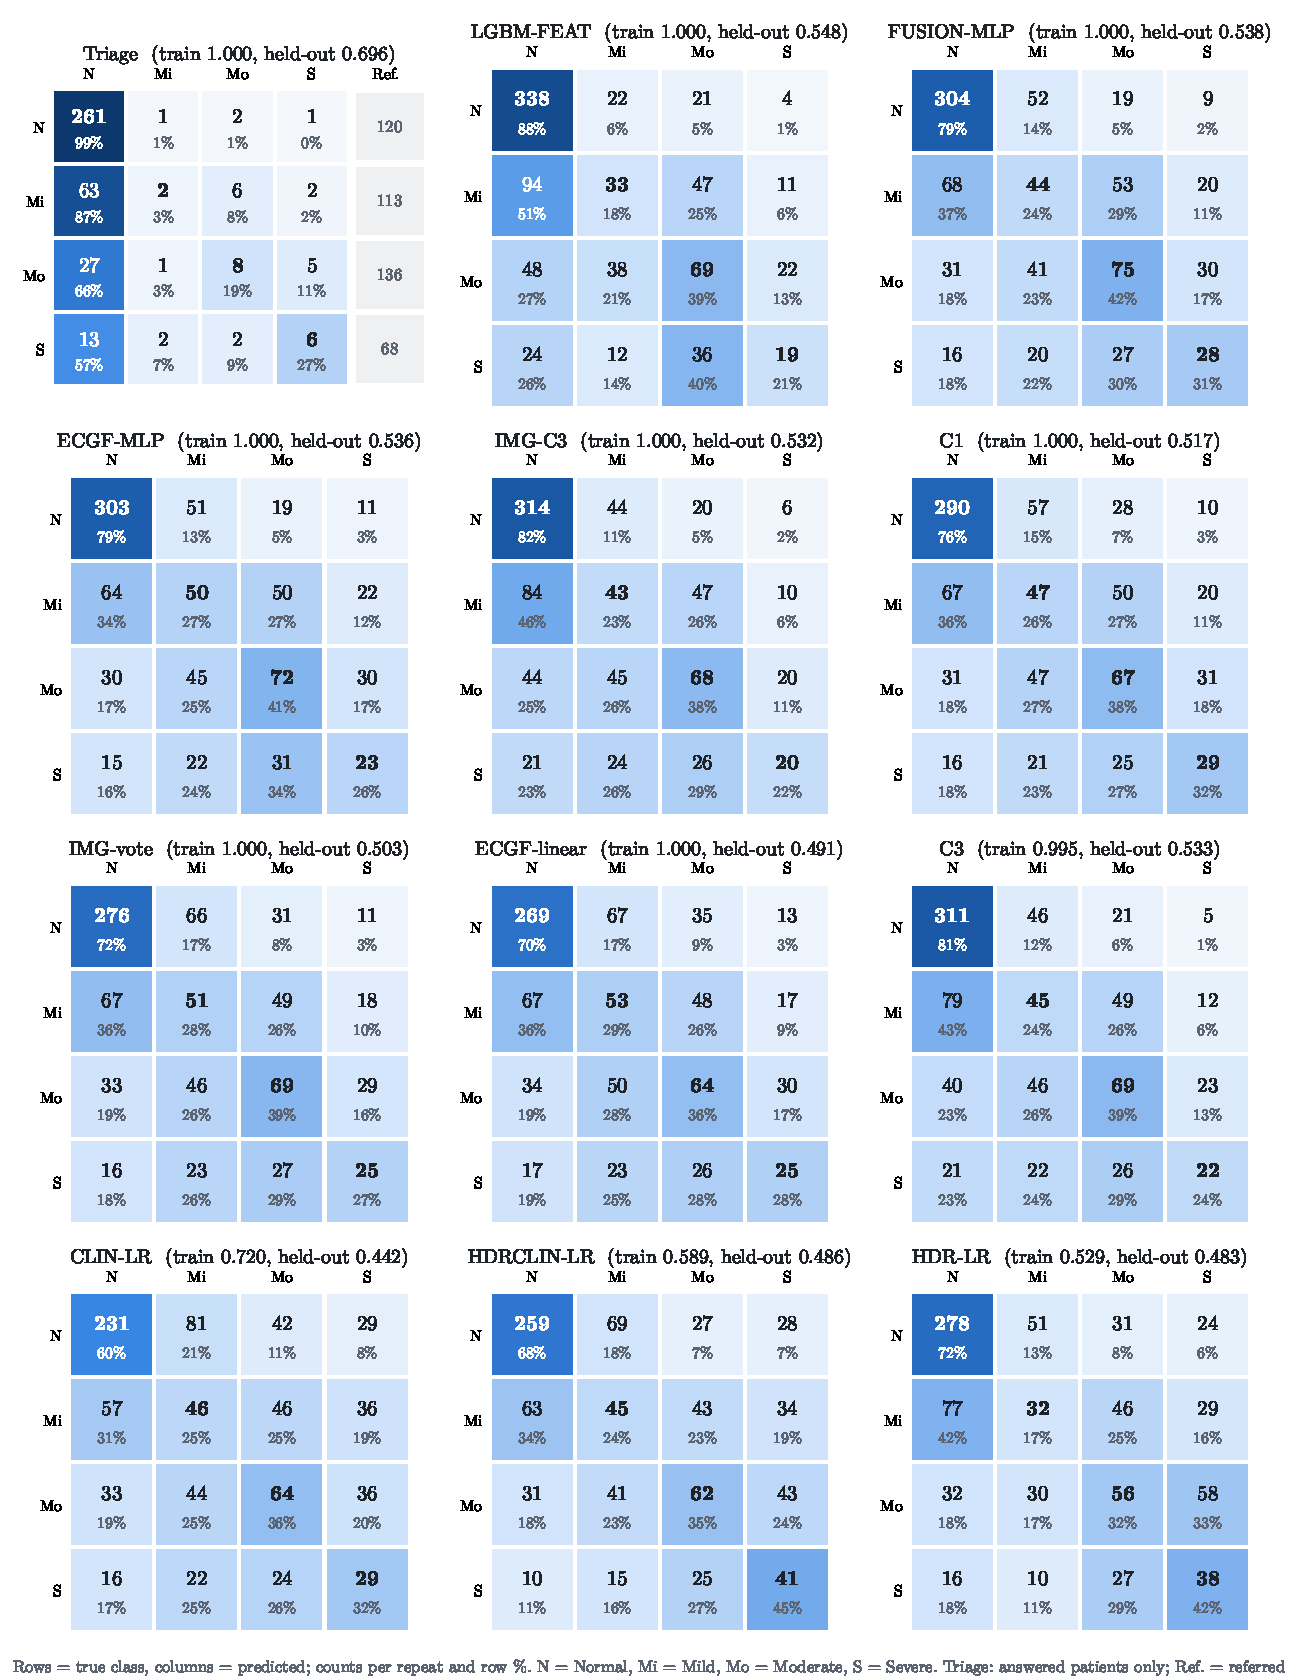
\includegraphics[width=1.00\linewidth,height=0.80\textheight,keepaspectratio]{figures/fig_6_1}
\caption{Held-out confusion matrices of the twelve main models, sorted by training accuracy (development cross-validation). Rows are the true class and columns the predicted class; counts are per repeat (each of the 837 ECGs is predicted once per repeat) and the colour is the row percentage (recall). Triage: answered patients only, with the referred patients in the last column.}\label{fig:6.1}
\end{figure}

Tables~\ref{tab:6.2}--\ref{tab:6.4} list all 79 classification models, each with its epochs, its training accuracy and its held-out accuracy, sorted by training accuracy, and Figure~\ref{fig:6.2} shows the 35 four-class models scored on all patients side by side. 55 of the 79 reach at least 0.995 training accuracy, yet the four-class models stay at 0.35--0.56 on held-out patients and on the fixed validation split alike: for every four-class model with a training accuracy of 0.99 or more that is scored on all patients, the gap between training and held-out accuracy is 0.44--0.65. The models that stay below 0.99 in training are the logistic regressions, the EF-band models and the ensembles whose meta-learner is fitted on out-of-fold outputs. Figure~\ref{fig:6.1} shows where the errors go: Normal is found in 60--99 \% of cases, Moderate in 19--42 \%, Severe in 21--45 \% and Mild in only 3--29 \%. Figure~\ref{fig:6.3} sorts the main models by heart-failure screen AUC (reduced EF against Normal). Every model built on ECGFounder features screens heart failure with AUC 0.78--0.84 (ECGF-MLP 0.835, FUSION-MLP 0.831), and the logistic regressions on header or clinical features reach 0.77--0.79, so the foundation-model representation carries most of the signal.

\begin{table}[htbp]
\caption{All models trained to (nearly) 100 \% training accuracy: main models and variants of every phase, sorted by training accuracy (highest first), ties by held-out accuracy. Epochs: median over the 15 folds; solver / trees / iter. = models not trained in epochs; $^{b}$ epochs of the member FUSION-MLP; $^{c}$ epochs of the member ECGF-MLP; $^{\dagger}$ selective model, accuracies on the patients it answers; $^{\ddagger}$ two-class task (Mild against Moderate); $^{\circ}$ trained on EchoNext only (training accuracy on EchoNext); $^{*}$ numbers from the owner's own runs; n/r = not reported.}\label{tab:6.2}
\footnotesize\setlength{\tabcolsep}{3pt}
\begin{tabular}{>{\raggedright\arraybackslash\hspace{0pt}}p{\dimexpr 0.560\linewidth-2\tabcolsep\relax}>{\raggedright\arraybackslash\hspace{0pt}}p{\dimexpr 0.160\linewidth-2\tabcolsep\relax}>{\raggedright\arraybackslash\hspace{0pt}}p{\dimexpr 0.140\linewidth-2\tabcolsep\relax}>{\raggedright\arraybackslash\hspace{0pt}}p{\dimexpr 0.140\linewidth-2\tabcolsep\relax}}
\toprule
\textbf{Model} & \textbf{Epochs (median)} & \textbf{Training acc.} & \textbf{Held-out acc.} \\
\midrule
\multicolumn{4}{>{\raggedright\arraybackslash\hspace{0pt}}p{\dimexpr\linewidth-2\tabcolsep\relax}}{\textit{Main models, development cross-validation (held-out accuracy)}} \\
Image-only triage (AGT-img)$^{\dagger}$ & 4,000 trees & 1.000 & 0.696 \\
LGBM-FEAT (LightGBM, header + engineered features) & 2,000 trees & 1.000 & 0.548 \\
FUSION-MLP (header + ECGFounder, MLP head) & 112 & 1.000 & 0.538 \\
ECGF-MLP (ECGFounder + MLP head) & 108 & 1.000 & 0.536 \\
IMG-C3 (IMG-vote + nested prior rule) & 108$^{c}$ & 1.000 & 0.532 \\
C1 (vote: FUSION-MLP, ECGF-linear, HDRCLIN-LR) & 112$^{b}$ & 1.000 & 0.517 \\
IMG-vote (image-only vote: ECGF-MLP, ECGF-linear) & 108$^{c}$ & 1.000 & 0.503 \\
ECGF-linear (ECGFounder + linear head) & 100 iter. & 1.000 & 0.491 \\
MMCLEAN selective model$^{\dagger\,*}$ (answers 7 \%) & n/r & 0.999 & 0.699 \\
C3 (C1 + nested prior rule) & 112$^{b}$ & 0.995 & 0.533 \\
CLIN-LR (image-only clinician features, logistic regression) & solver & 0.720 & 0.442 \\
HDRCLIN-LR (header + clinical features, logistic regression) & solver & 0.589 & 0.486 \\
HDR-LR (header measurements, logistic regression) & solver & 0.529 & 0.483 \\
\multicolumn{4}{>{\raggedright\arraybackslash\hspace{0pt}}p{\dimexpr\linewidth-2\tabcolsep\relax}}{\textit{Variants of every phase, development cross-validation (held-out accuracy)}} \\
E2 LightGBM, features + ECGFounder PCA & 2,000 trees & 1.000 & 0.557 \\
ENH-vote (6 members, tuned class weights) & 108$^{c}$ & 1.000 & 0.549 \\
ULT M9 $k$-nearest neighbours ($k$ = 15) & none (kNN) & 1.000 & 0.546 \\
E1 MLP, header + ECGFounder + feature families & 64 & 1.000 & 0.542 \\
ULT M10 gradient boosting & 2,000 iter. & 1.000 & 0.540 \\
Multitask MLP (class + EF) & 131 & 1.000 & 0.536 \\
HIER two-stage (Normal / middle / Severe, then Mild vs Moderate) & 108$^{c}$ & 1.000 & 0.535 \\
E7 mixup MLP & 144 & 1.000 & 0.534 \\
ENH M5 logistic regression on the HIER inputs & solver & 1.000 & 0.501 \\
ENH M2 synthetic 10-s ECG $\rightarrow$ ECGFounder & solver & 1.000 & 0.489 \\
ENH M4 MiniRocket & solver & 1.000 & 0.469 \\
ENH M3 median-beat shape model & solver & 1.000 & 0.412 \\
ULT M8 logistic regression, multi-scale ECGFounder & solver & 1.000 & 0.496 \\
E4 hierarchical MLP & 52 / 39 & 0.999 & 0.540 \\
E6 signal-quality gating & 112$^{b}$ & 0.988 & 0.542 \\
E3 weighted average of the C1 members & 112$^{b}$ & 0.985 & 0.530 \\
E3 stacking (logistic meta-learner) & 112$^{b}$ & 0.826 & 0.532 \\
ULT-stack (10 members + predicted EF) & 108$^{c}$ & 0.794 & 0.537 \\
SUPER-TOP10-ORD, hospital-trained members only & 108$^{c}$ & 0.783 & 0.539 \\
ULT M12 zone logistic regression & solver & 0.624 & 0.349 \\
ENH M6 EF ridge $\rightarrow$ EF bands & exact & 0.557 & 0.477 \\
\bottomrule
\end{tabular}
\end{table}


\begin{table}[htbp]
\caption{All models trained to (nearly) 100 \% training accuracy: label studies and networks on the fixed split, sorted by training accuracy (highest first), ties by held-out accuracy. Symbols as in Table~\ref{tab:6.2}.}\label{tab:6.3}
\footnotesize\setlength{\tabcolsep}{3pt}
\begin{tabular}{>{\raggedright\arraybackslash\hspace{0pt}}p{\dimexpr 0.560\linewidth-2\tabcolsep\relax}>{\raggedright\arraybackslash\hspace{0pt}}p{\dimexpr 0.160\linewidth-2\tabcolsep\relax}>{\raggedright\arraybackslash\hspace{0pt}}p{\dimexpr 0.140\linewidth-2\tabcolsep\relax}>{\raggedright\arraybackslash\hspace{0pt}}p{\dimexpr 0.140\linewidth-2\tabcolsep\relax}}
\toprule
\textbf{Model} & \textbf{Epochs (median)} & \textbf{Training acc.} & \textbf{Held-out acc.} \\
\midrule
\multicolumn{4}{>{\raggedright\arraybackslash\hspace{0pt}}p{\dimexpr\linewidth-2\tabcolsep\relax}}{\textit{Label-quality studies, C3 recipe (accuracy on the subset in brackets)}} \\
NF: noise-free training (all classes) [264 clean, clear-cut ECGs] & 45$^{b}$ & 1.000 & 0.673 \\
HC30: train on exact-name links within 30 days [395 reliable links] & 52$^{b}$ & 1.000 & 0.583 \\
CLEAR: train without the 255 border ECGs [582 clear-cut ECGs] & 104$^{b}$ & 0.993 & 0.670 \\
VER: 15 labels corrected to a high-confidence echo [all 837] & 132$^{b}$ & 0.986 & 0.537 \\
NFS: noise-free training, Severe kept [264 clean, clear-cut ECGs] & 44$^{b}$ & 0.985 & 0.694 \\
MMCLEAN: drop 217 suspect Mild or Moderate labels [620 kept ECGs] & 95$^{b}$ & 0.978 & 0.669 \\
\multicolumn{4}{>{\raggedright\arraybackslash\hspace{0pt}}p{\dimexpr\linewidth-2\tabcolsep\relax}}{\textit{Image and signal networks, fixed split (validation accuracy)}} \\
XGBoost (waveform features) & 2,000 trees & 1.000 & 0.494 \\
HOG + RBF-SVM & solver & 1.000 & 0.423 \\
EfficientNet-B0 & 37 & 1.000 & 0.417 \\
1-D SE-ResNet & 32 & 0.999 & 0.435 \\
ECGNet & 21 & 0.999 & 0.435 \\
MobileNetV3-Large & 57 & 0.999 & 0.387 \\
ResNet-18 & 24 & 0.997 & 0.423 \\
ECGFounder fine-tuned (stages 5--6) & 12 & 0.996 & 0.560 \\
ConvNeXt-Atto & 53 & 0.996 & 0.345 \\
Header 0.6 + ResNet-18 0.4 & 24 (ResNet-18) & 0.972 & 0.458 \\
Logistic regression (header) & solver & 0.674 & 0.405 \\
\bottomrule
\end{tabular}
\end{table}


\begin{table}[htbp]
\caption{All models trained to (nearly) 100 \% training accuracy: the run with EchoNext, sorted by training accuracy (highest first), ties by held-out accuracy. Symbols as in Table~\ref{tab:6.2}.}\label{tab:6.4}
\footnotesize\setlength{\tabcolsep}{3pt}
\begin{tabular}{>{\raggedright\arraybackslash\hspace{0pt}}p{\dimexpr 0.560\linewidth-2\tabcolsep\relax}>{\raggedright\arraybackslash\hspace{0pt}}p{\dimexpr 0.160\linewidth-2\tabcolsep\relax}>{\raggedright\arraybackslash\hspace{0pt}}p{\dimexpr 0.140\linewidth-2\tabcolsep\relax}>{\raggedright\arraybackslash\hspace{0pt}}p{\dimexpr 0.140\linewidth-2\tabcolsep\relax}}
\toprule
\textbf{Model} & \textbf{Epochs (median)} & \textbf{Training acc.} & \textbf{Held-out acc.} \\
\midrule
\multicolumn{4}{>{\raggedright\arraybackslash\hspace{0pt}}p{\dimexpr\linewidth-2\tabcolsep\relax}}{\textit{Run with EchoNext on the owner's computer$^{*}$ (hospital held-out accuracy)}} \\
EN-MiMo-GBM (Mild vs Moderate)$^{\circ}$$^{\ddagger}$ & n/r & 1.000 & 0.586 \\
EN-MiMo-LR (Mild vs Moderate)$^{\circ}$$^{\ddagger}$ & n/r & 1.000 & 0.577 \\
H-MiMo-GBM (Mild vs Moderate)$^{\ddagger}$ & n/r & 1.000 & 0.569 \\
H-TAB-GBM & n/r & 1.000 & 0.548 \\
M9 & n/r & 1.000 & 0.546 \\
H-X-GBM & n/r & 1.000 & 0.546 \\
EN-gbm-X$^{\circ}$ & n/r & 1.000 & 0.539 \\
M10 & n/r & 1.000 & 0.539 \\
EN-gbm$^{\circ}$ & n/r & 1.000 & 0.522 \\
M5 & n/r & 1.000 & 0.507 \\
ECGF-lin & n/r & 1.000 & 0.498 \\
M8 & n/r & 1.000 & 0.496 \\
EN-cls$^{\circ}$ & n/r & 1.000 & 0.479 \\
H-TAB-LR & n/r & 1.000 & 0.473 \\
M12 & n/r & 1.000 & 0.346 \\
PIX-ZS (pixel CNN, EchoNext printouts)$^{\circ}$ & n/r & 0.999 & 0.505 \\
EN-cls-all$^{\circ}$ & n/r & 0.999 & 0.490 \\
EN-mu-mid$^{\circ}$ & n/r & 0.999 & 0.409 \\
ECGF-MLP & n/r & 0.996 & 0.536 \\
EN-cls-all-X$^{\circ}$ & n/r & 0.996 & 0.497 \\
PIX-ZS-band (pixel CNN, EF bands)$^{\circ}$ & n/r & 0.929 & 0.492 \\
EN-band-all$^{\circ}$ & n/r & 0.820 & 0.458 \\
SUPER ensemble & n/r & 0.790 & 0.552 \\
EN-band$^{\circ}$ & n/r & 0.781 & 0.479 \\
SUPER-TOP10-ORD ensemble & n/r & 0.748 & 0.558 \\
STAGED-4 ensemble & n/r & 0.722 & 0.548 \\
M6 (EF bands) & n/r & 0.557 & 0.477 \\
EF-band & n/r & -- & 0.479 \\
\bottomrule
\end{tabular}
\end{table}


\begin{figure}[htbp]
\centering
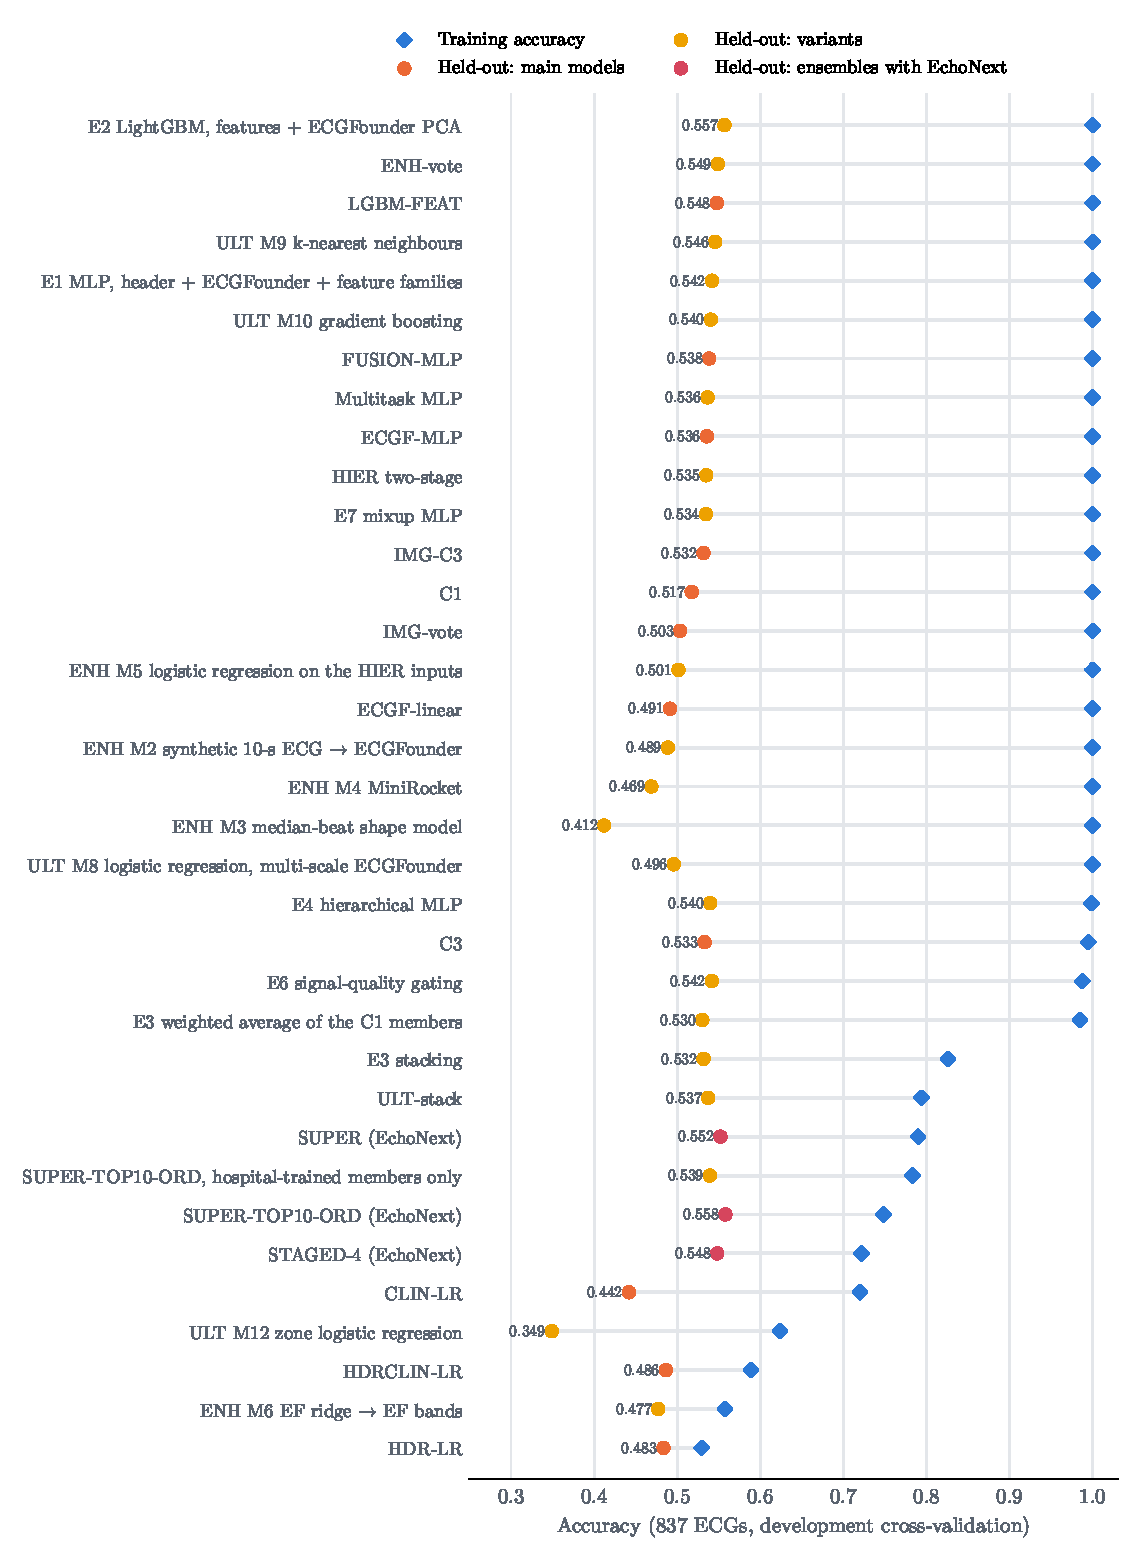
\includegraphics[width=0.97\linewidth,height=0.86\textheight,keepaspectratio]{figures/fig_6_2}
\caption{The 35 four-class models scored on all 837 ECGs in development cross-validation (main models, variants and the ensembles with EchoNext members), sorted by training accuracy (highest at the top): training accuracy (blue diamonds) against held-out accuracy (coloured by group, value at the left).}\label{fig:6.2}
\end{figure}

\begin{figure}[htbp]
\centering
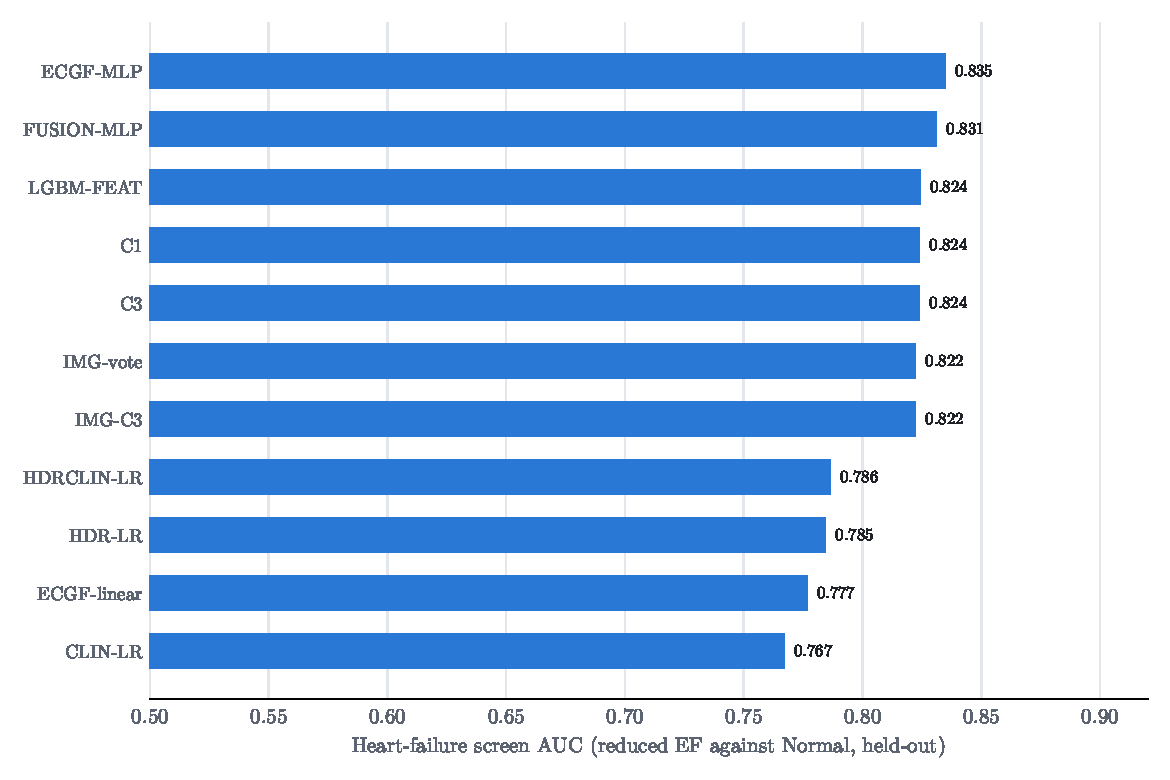
\includegraphics[width=0.85\linewidth,height=0.80\textheight,keepaspectratio]{figures/fig_6_3}
\caption{Heart-failure screen AUC (reduced EF against Normal) of the main models after training to (nearly) 100 \% training accuracy (held-out, development cross-validation). C3 and IMG-C3 share the probabilities of C1 and IMG-vote.}\label{fig:6.3}
\end{figure}

\section{Results in the upper 50s and the 60s}\label{sec:6.3}

Figure~\ref{fig:6.4} groups the results by the population they are scored on.

\begin{itemize}
  \item \textbf{All patients (development cross-validation).} Three results reach 0.55 or more: SUPER-TOP10-ORD (0.558), E2 LightGBM (0.557) and the greedy SUPER ensemble (0.552). Several independent model families reach 0.54--0.55, so the level is reproducible.
  \item \textbf{Answered patients.} The triage model rises into the upper 60s (0.696 on 48 \%): the models' confidence is informative.
  \item \textbf{Clean or reliable labels.} Where the labels are reliable, the same recipe scores 0.583--0.694.
  \item \textbf{Fixed split.} On the 168 validation ECGs, fine-tuned ECGFounder reaches 0.560 and every other network 0.35--0.49.
\end{itemize}

\begin{figure}[htbp]
\centering
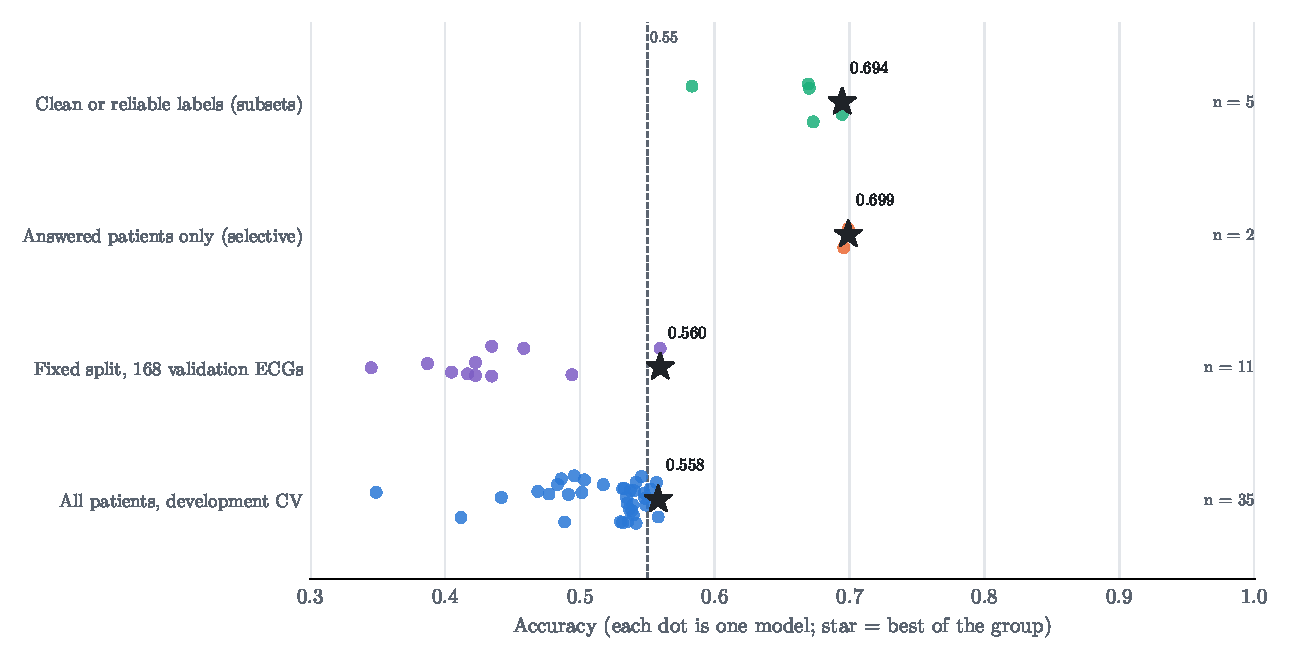
\includegraphics[width=0.97\linewidth,height=0.80\textheight,keepaspectratio]{figures/fig_6_4}
\caption{Every result after training to (nearly) 100 \% training accuracy, grouped by evaluation population (each dot is one model; stars mark the best of each group).}\label{fig:6.4}
\end{figure}

\section{Trade-off analysis}\label{sec:6.4}

\begin{figure}[htbp]
\centering
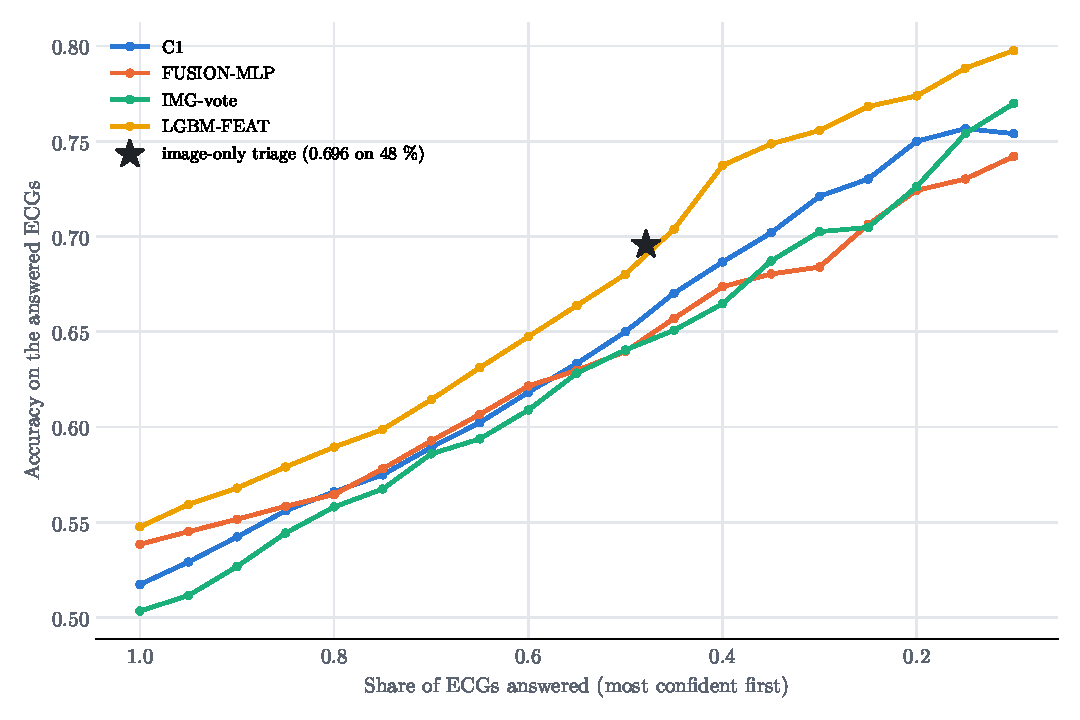
\includegraphics[width=0.75\linewidth,height=0.80\textheight,keepaspectratio]{figures/fig_6_5}
\caption{Accuracy against the share of ECGs answered, most confident first (held-out, development cross-validation; descriptive, the confidence cut-off is not nested), with the triage model as a star.}\label{fig:6.5}
\end{figure}

\textbf{Coverage against accuracy.} Answering fewer, more confident patients raises accuracy steadily (Figure~\ref{fig:6.5}). For LightGBM, accuracy rises from 0.548 on all ECGs to 0.680 on the most confident half and 0.768 on the most confident quarter; for C1 from 0.517 to 0.650 and 0.730. The triage model sits at 48 \% coverage and 0.696.

\textbf{Mild detected against accuracy.} Figure~\ref{fig:6.6} plots accuracy against Mild recall for the four-class models. Giving the Mild class more weight moves a model along a curve: IMG-vote goes from 0.503 at Mild recall 0.28 to 0.420 at 0.57. The most accurate models find only 13--24 \% of the Mild ECGs. The triage results reach the upper 60s by leaving the Mild band, the class that echo itself places least reliably, to a second reading.

\begin{figure}[htbp]
\centering
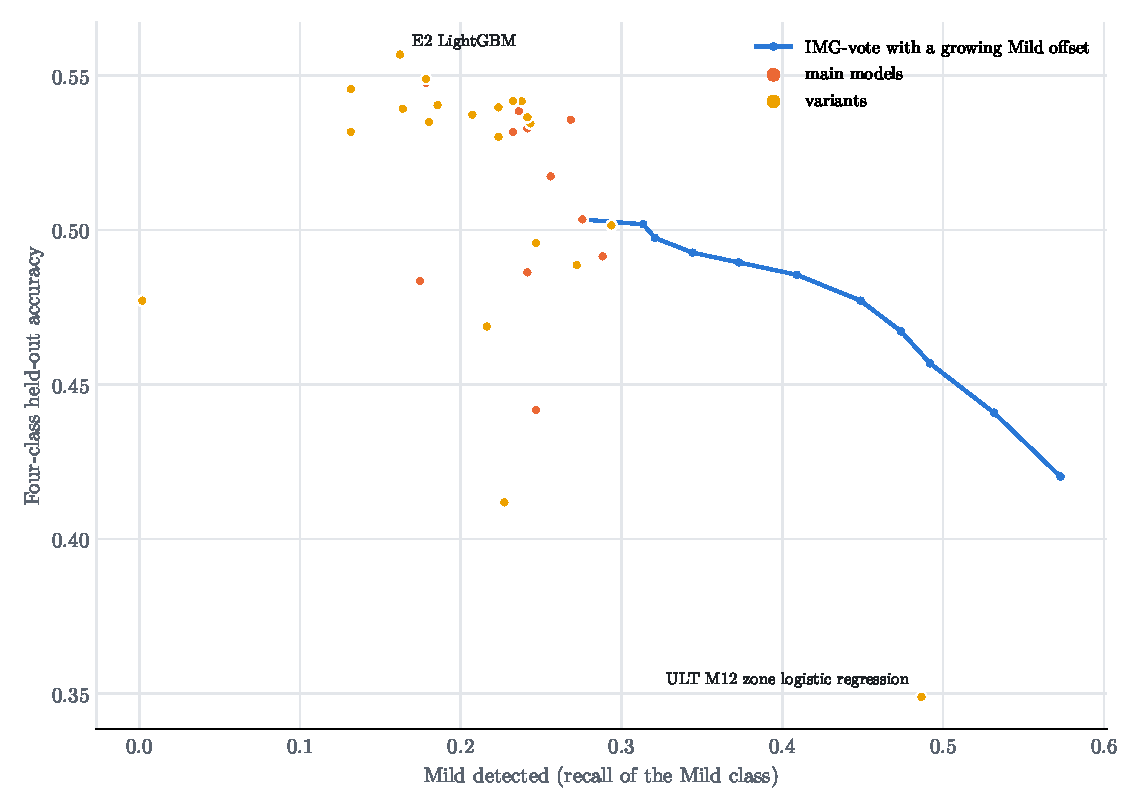
\includegraphics[width=0.85\linewidth,height=0.80\textheight,keepaspectratio]{figures/fig_6_6}
\caption{Mild detected (recall of the Mild class) against four-class held-out accuracy for the main models and the variants after training to (nearly) 100 \% training accuracy. The line shows the effect of a growing Mild weight on IMG-vote.}\label{fig:6.6}
\end{figure}

\section{Why the results are strong and why higher accuracy is not feasible}\label{sec:6.5}

Every model family, label-cleaning scheme and evaluation lands within a few points of the same level, whether the model fits its training data perfectly or not. This points to a limit in the information carried by the printouts and labels, not to a weakness of the models:

\begin{itemize}
  \item \textbf{EF precision against band width.} Our best EF regressor errs with SD $\approx$ 13.7 points ($r=0.624$), which for these class bands gives 0.580 for a perfect grader; our best model reaches 0.558. Seventy per cent would need SD $\le$ 7.7, i.e. $r\approx$ 0.90, beyond any published AI-ECG model (Figure~\ref{fig:6.7}).
  \item \textbf{Errors sit at the class limits.} 50 \% of the ECGs have an echo EF within 6 points of a limit. They are misclassified 64--67 \% of the time, while ECGs at least 10 points from every limit are graded with 75--76 \% accuracy (Figure~\ref{fig:6.8}).
  \item \textbf{The ECG separates extremes, not neighbours.} For the vote ensemble C1, pairwise AUROCs are 0.89 for Normal against Severe and 0.86 against Moderate, but 0.75 for Normal against Mild, 0.65 for Mild against Moderate and 0.58 for Moderate against Severe.
  \item \textbf{Label consistency.} 6.6 \% of the labels disagree with their own echo EF band, and repeat echoes of the same patient differ by a median of 15.4 EF points.
\end{itemize}
\begin{figure}[htbp]
\centering
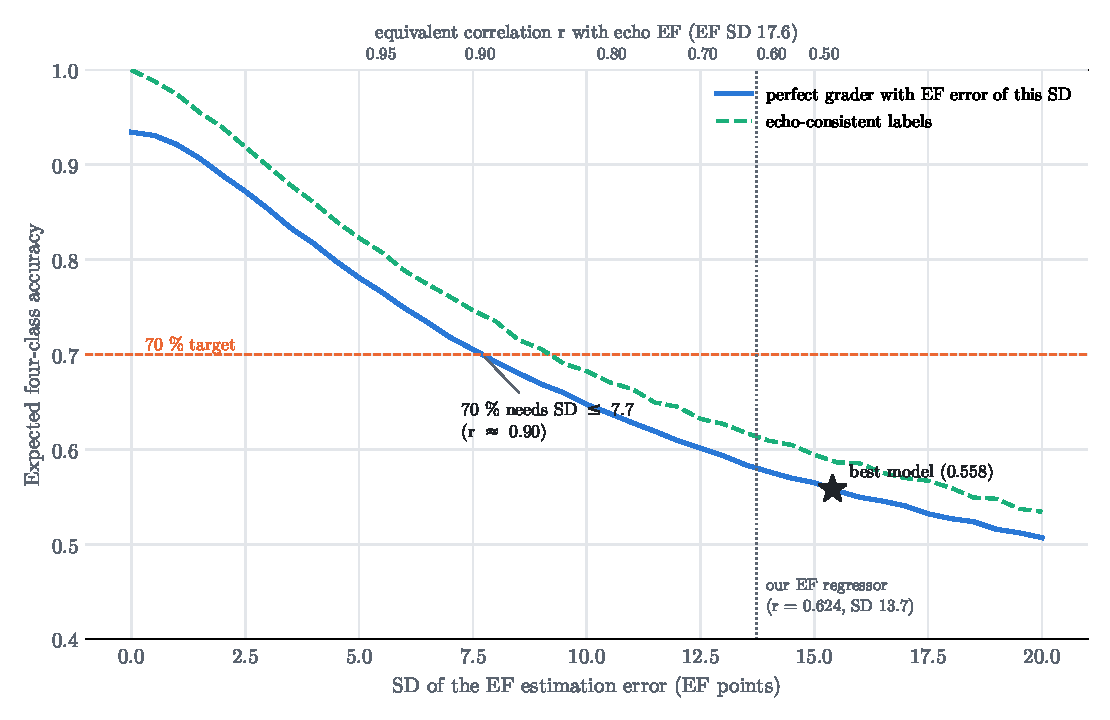
\includegraphics[width=0.80\linewidth,height=0.80\textheight,keepaspectratio]{figures/fig_6_7}
\caption{Expected four-class accuracy against the SD of the EF estimation error (simulation on the 837 development ECGs, recorded and echo-consistent labels). The star marks the best model (0.558); the dotted line marks our best EF regressor.}\label{fig:6.7}
\end{figure}

\begin{figure}[htbp]
\centering
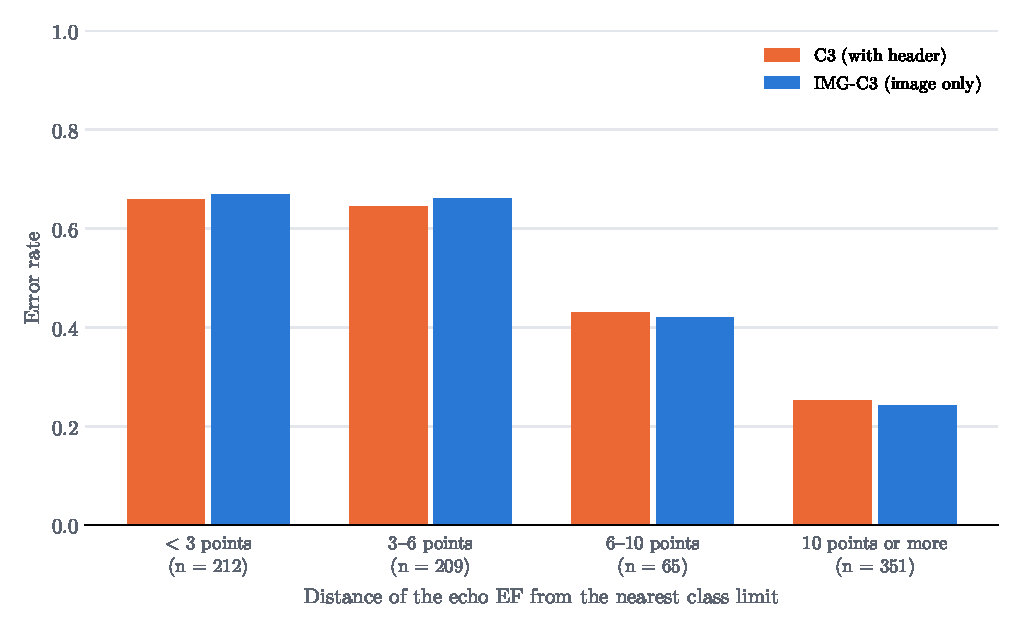
\includegraphics[width=0.70\linewidth,height=0.80\textheight,keepaspectratio]{figures/fig_6_8}
\caption{Error rate of C3 and IMG-C3 (trained to 100 \%) by distance of the echo EF from the nearest class limit (held-out, development cross-validation).}\label{fig:6.8}
\end{figure}

\begin{itemize}
  \item \textbf{Input format and size.} A printout shows each lead for only 2.5 s, and 837 training ECGs are few for networks with millions of parameters: every such network memorises its training ECGs (Figure~\ref{fig:3.2}).
\end{itemize}
Exceeding 0.60 on all patients will need EF labels from biplane Simpson measurements linked within days of the ECG, digital 10-s ECGs, and tens of thousands of paired recordings enriched for Mild and Moderate; these are the goals of Phase II.
